\documentclass[tikz,border=5mm]{standalone}
\begin{document}
	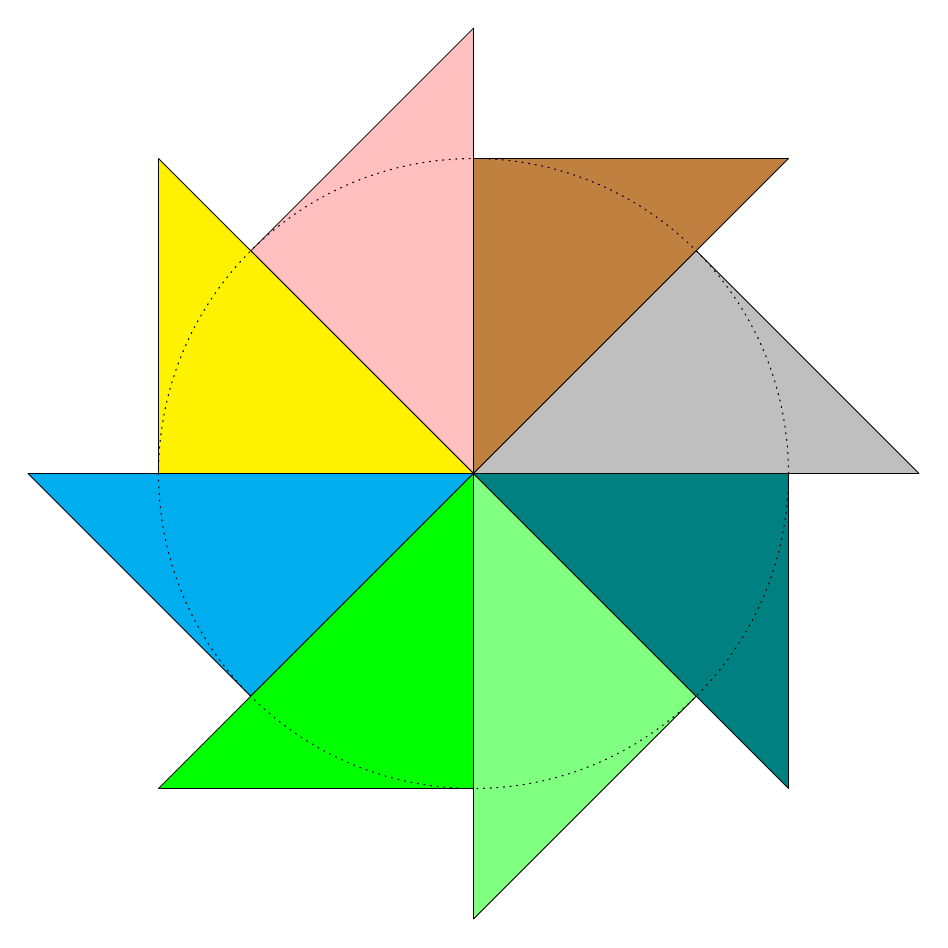
\begin{tikzpicture}[line cap=round,line join=round]
		\def\r{4}
		\foreach \mau/\gocxoay in {brown/0,pink/45,yellow/90,cyan/135,green/180,green!50/225,teal/270,gray!50!white/315}
		\draw[fill=\mau,rotate=\gocxoay,line width=.3pt] (0,0)--(0,\r)--++(\r,0)--cycle;
		\draw[dotted,black] (0,0) circle(\r);
	\end{tikzpicture}
\end{document}